\subsection{FRET спектроскопия и микроскопия}
%\todo{2S Из файла Armeev\_disser.pdf - со стр. 23 весь п. 1.4 с картинками. НО - нужно весь текст переписать так, чтобы его не детектировал антиплагиат - нужно чтобы подряд не было 3 похожих слов (!) можно перефоразировать, заменять на синонимы, менять местами слова}
%то есть до страницы 36 включительно?


\subsubsection{Ферстеровский резонансный перенос энергии}

    Ферстеровский резонансный перенос энергии (Forster resonance energy transfer, FRET) это эффект безызлучательного переноса энергии с одного красителя-флуорофора на другой. Пару (или более) флуорофоров подбирают таким образом, чтобы спектр поглощения акцептора перекрывался со спектром флуоресценции донора. Флуорофоры могут быть пришиты к аминокислотам или азотистым основаниям ДНК с помощью различных линкерных молекул. По определение эффективность FRET - это отношение вероятности переноса энергии с донора на акцептор по отношению ко всем другим переходам в расчете на событие возбуждение донора:
\begin{equation}
    E_{FRET} = \frac{k_\text{ET}}{k_f + k_\text{ET} + \sum{k_i}}
\end{equation}    
 где $k_{ET}$ - скорость переноса энергии с донора на акцептор, $k_f$ - скорость процесса флуоресценции донора,  $k_i$ - скорости других неизлучательных процессов релаксации донора, за исключением переноса энергии на акцептор.
    Эффективность переноса энергии существенно зависит от расстояния между метками и может быть описана следующей формулой:

\begin{equation}
    E_{FRET}=\frac{1}{1+(R/R_0)^6}
    \label{fret_E}
\end{equation}
    где R - расстояние между метками, $R_0$ - радиус
     Ферстера, расстояние между метками, отвечающее 50\% эффективности переноса энергии между флуорофорами (см. Рис. \ref{fig:p1_5_fret:f3}). Согласно данной формуле, измеряя эффективность FRET возможно вычислить расстояние между участками меченой макромолекулы. Для каждой пары меток радиус Ферстера индивидуален, он зависит от ряда факторов, в том числе от квантового выхода флуоресценции донора, ориентации красителя на поверхности молекулы (ориентационный фактор), коэффициента преломления среды и т.д. 

\begin{figure} [h!]
    \centering
    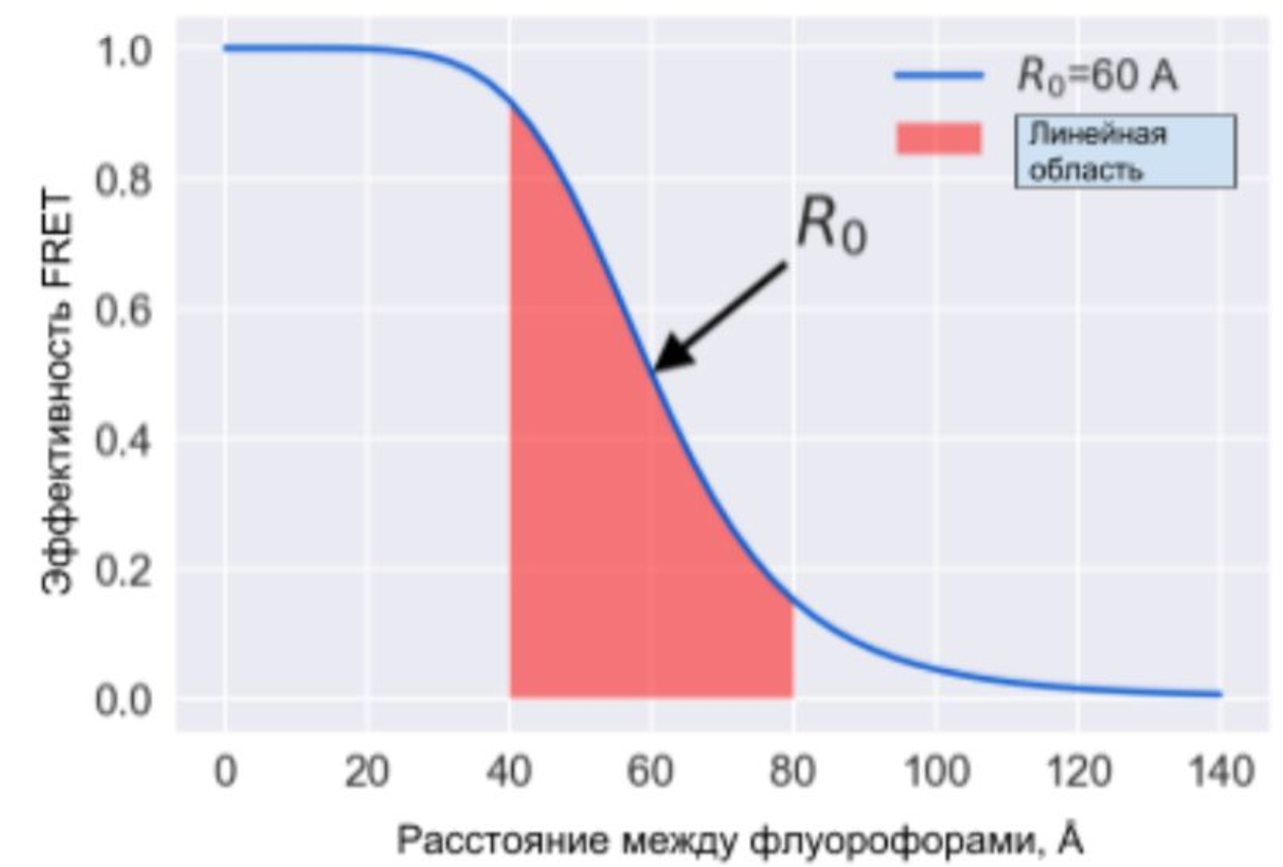
\includegraphics[width=\textwidth]{images/p1/part1_5_fret/part1_5_fret_f3.pdf}
    \caption[Зависимость эффективности переноса энергии от расстояния между флуорофорами.]{Зависимость эффективности переноса энергии от расстояния. Стрелкой показана величина Ферстеровского радиуса. Красным показана область изменений, близкая к линейной. }
    \label{fig:p1_5_fret:f3}
\end{figure}

    Эффективность переноса энергии может быть выражена через отношение времен жизни флуоресценции донора в отсутствии и присутствии акцептора:
\begin{equation}
    E_{FRET}= 1-\tau_{D}^{'}/\tau_D
\end{equation}
    где $\tau_{D}^{'}$ - время жизни флуоресценции донора в присутствии акцептора,  $\tau_D$ время жизни донора в отсутствии акцептора.
    
    Альтернативным является выражение эффективности переноса через величины интенсивности флуоресценции донора и акцептора:
    
\begin{equation}
   E_{FRET}=\frac{F_A}{F_A+\gamma F_D}
   \label{eq:p1:fret}
\end{equation}
    где $F_A= I_A - B_A - \alpha_{DA} (I_D - B_D) - D_{ex}$, $F_D = I_D - B_D - \alpha_{AD} (I_A - B_A )$ и 
В последних формулах $I_A$ и $I_D$  - регистрируемые интенсивности сигнала акцептора и донора, соответственно; $B_A$ и $ B_D$ - уровни фонового сигнала в канале акцептора и донора, соответственно;  $\alpha_{DA}$ и $\alpha_{AD}$ - перекрестные коэффициенты (crosstalk coefficients), характеризующие долю флуоресценции донора, регистрируемую в канале акцептора ( $\alpha_{DA}$ ), и долю излучения акцептора, регистрируемую в канале донора ( $\alpha_{AD}$ ). Поправочные коэффициенты помогают учитывать особенности  оптической схемы конфокального микроскопа или спектрофлуориметра, для разных пар флуоресцентных меток они отличаются. $D_{ex}$ - это величина сигнала прямого возбуждения акцептора (возникающая в следствие возможного поглощения фотонов акцептором на длине волны поглощения донора). $\gamma$ - так называемый фактор детекции, он позволяет учитывать различия в эффективностях детекции флуоресценции $(\eta)$ донора и акцептора и различия в их квантовых выходах флуоресценции ($\Phi$) \cite{dahan_ratiometric_1999}. Фактор детекции может быть представлен в виде:

\begin{equation}
    \gamma = \gamma_{instrument} \gamma_{dye} = \frac{\eta_A \Phi_A}{\eta_D \Phi_D}
\end{equation}
где $\Phi$ - квантовый выход, $\eta$ - эффективность детекции.
    Эффективность детекции флуоресценции зависит от спектральной чувствительности детекторов (лавинных фотодиодов или фотоэлектронных умножителей) и спектральных характеристик оптических элементов, через которые проходит сигнал от образца. 
    Измерение фактора детекции в ряде случаев может быть затруднено и его принимают за единицу. В таком случае измеряемая по формуле (\ref{eq:p1:fret}) величина является не истинным коэффициентом переноса, такую величину называют ``коэффициентом близости'' (PR - proximity ratio). Коэффициент близости нельзя непосредственно связать с расстоянием между флуоресцентными метками, однако, используя этот коэффициент можно делать выводы о гетерогенности образца, и о качественных эффектах сближения или удаления частиц.

\subsubsection{Детекция сигнала от одиночных молекул}
    Эффективность FRET может быть измерена в объеме сразу от многих частиц при помощи прибора спектрофлуориметра. В этом случае измеренный сигнал соответствует некоторому среднему сигналу от ансамбля молекул \cite{klose_simulation_2012}. Такой усредненный сигнал может не соответствовать ни одному конкретному состоянию системы на молекулярном уровне, а являться суперпозицией нескольких состояний разных частиц. Чтобы добиться связи сигнала FRET с конкретными состояниями молекулярной системы, необходимо, как минимум, измерять эффективности FRET у одиночных частиц, такой метод называется spFRET (single particle FRET). С помощью метода spFRET возможно оценивать как средние расстояния \cite{okumus_vesicle_2004}, так и временную динамику изменения расстояний между метками \cite{li_rapid_2005}. Вопрос заключается в том, каким образом снимать сигнал от одной частицы. Одни вариант заключается в иммобилизации частиц на поверхности. Иммобилизовав частицы, можно использовать подходы, основанные на эффекте полного внутреннего отражения, которые позволяют проводить измерения в тонком слое частиц у поверхности \cite{roy_practical_2008}. Преимущество такого метода в возможности наблюдения эволюции сигнала сразу для многих частиц в поле зрения микроскопа. Недостатком является возможные взаимодействия частиц с подложкой, которые могут повлиять на их структуру и динамику \cite{zanetti-domingues_hydrophobic_2013}. Альтернативных подход основан на измерении флуоресценции от единичных молекул, свободно диффундирующих сквозь фокальный объем конфокального флуоресцентного микроскопа (см. Рис. \ref{fig:p1_5_fret:f4}). Для реализации этого метода необходимо, чтобы исследуемые частицы находились в достаточно низкой концентрации, чтобы одновременно в фокальном объеме находилось не более одной частицы. Метод требует наличия конфокального микроскопа, чувствительных лавинных фотодиодов (APD или SAPD). По мере проплывания частиц можно собирать необходимую статистику, однако поскольку проплывание обычно занимает миллисекунды, присутствуют ограничения на возможности слежения за динамикой процессов внутри частицы. 

\begin{figure} [h!]
    \centering
    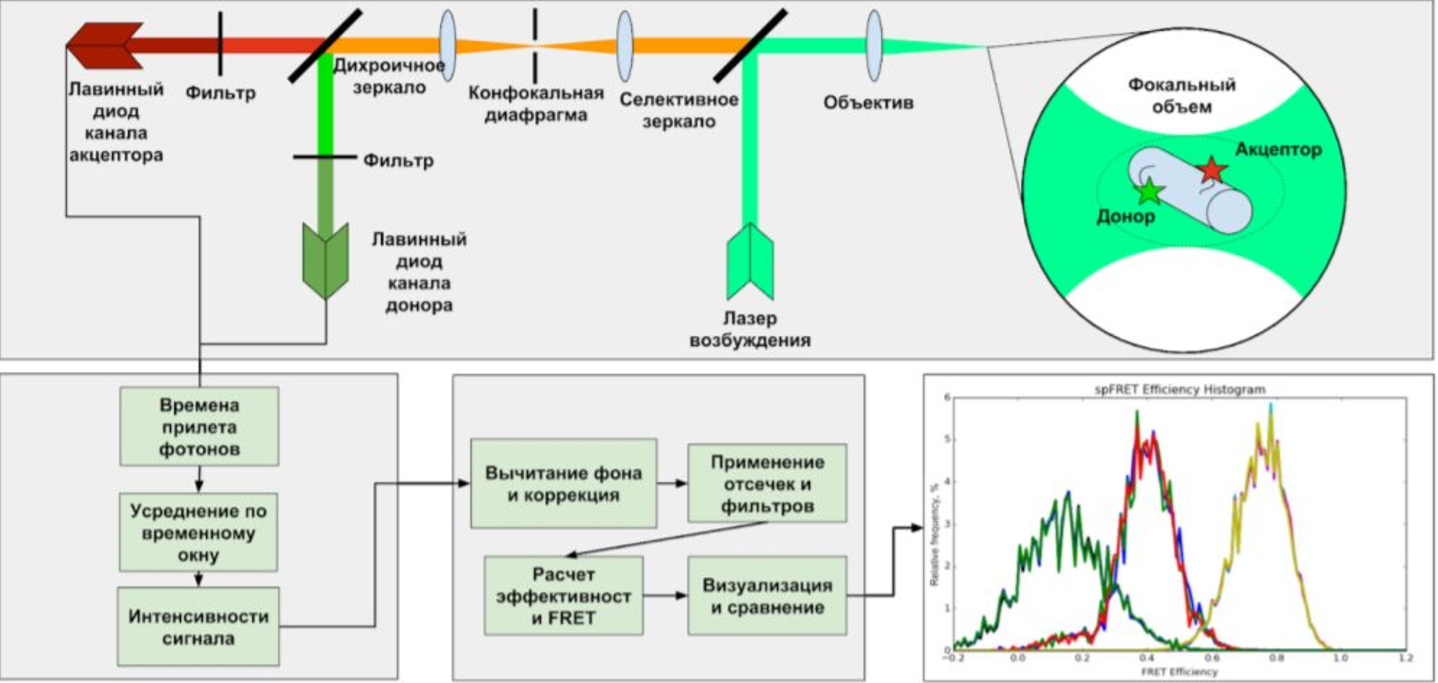
\includegraphics[width=\textwidth]{images/p1/part1_5_fret/part1_5_fret_f4.pdf}
    \caption[Схема экспериментов spFRET]{Схема экспериментов spFRET. Один лазер возбуждает флуоресценцию. Флуоресценция из конфокального объема собирается на лавинных фотодиодах. Времена прилета фотонов анализируются программным обеспечением микроскопа, либо специализированным ПО.}
    \label{fig:p1_5_fret:f4}
\end{figure}


\subsubsection{Подходы к измерению эффективности FRET}
Величина $E_{FRET}$, как следует из вышеприведенных формул, может быть рассчитана двумя способами, либо через время флуоресценции донора \cite{sisamakis_accurate_2010}, либо через измерение интенсивностей свечения донора и акцептора. Последний подход называется ратиометрическим подходом. 

Для того, чтобы измерить времена флуоресценции необходимо существенно более сложное оборудование. Порядок времен флуоресценции составляет порядка наносекунд, поэтому требуются лазерные источники и синхронизированные детекторы, способные работать в пикосекундном диапазоне. Такой подход реализован в методе TCSPC (Time Correlated Single Photon Counting). Он же используется в популярном методе микроскопии супер разрешения FLIM (fluorescence-lifetime imaging microscopy).
Важным преимуществом данного метода является отсутствие необходимости учитывать эффекты, связанные с мощностью осветителя, различными параметрами оптической системы и системы детекции, влияющими на корректировочные факторы. Наличие временного разрешения пикосекундрного диапазона, также позволяет эффективно проводить отсеивание шумовых всплесков в сигнале.

Ратиометрический подход может быть реализован с использованием более простого оборудования, например, конфокального микроскопа с лазером непрерывного излучения. Однако, этот подход чувствителен к шумовым эффектам, связанным с рассеянием света, колебаниям интенсивности лазера. Для соотнесения измеренных интенсивностей с реальными фотофизическими процессами необходимо предварительно измерить фактор детекции $\gamma$. Отдельной проблемой является то, что данный фактор может зависеть от конформационных изменений в молекулярной системе, так как квантовые выходы чувствительны к окружению флуорофоров.


\subsubsection{Подходы к измерению интенсивности флуоресценции spFRET от одиночных молекул}

Интенсивности флуоресценции в радиометрическом подходе, в зависимости от приборных возможностей, регистрируют либо в виде временного ряда, описывающего прилет отдельных фотонов (single photon counting), либо в виде некоторого сигнала, описывающего зависимость интенсивности от времени. В последнем случае прибор будет проводить усреднение (бинирование) сигнала с некоторым временным интервалом. В случае измерения spFRET в растворе, данный временной интервал необходимо выбирать с учетом кинетики проплывания частиц через фокальных объем микроскопа.
Для оценки времени проплывания частицы через фокальный объем можно использовать диффузионное соотношение:
 
\begin{equation}
    \tau \approx \langle x^2 \rangle / 2D
\end{equation}
    где $\tau$ - время проплывания, $D$ - коэффициент диффузии, $x$ - координата частицы вдоль одной из осей системы координат.
    
Для обработки непосредственно времен прилета фотонов также разработаны различные алгоритмы, позволяющие выделять внутри временного ряда события, связанные с проплыванием частиц и оценивать фоновых сигнал \cite{ingargiola_fretbursts_2016}. 
Оценку фонового сигнала можно проводить непосредственно анализируя правый край гистограммы распределения временных задержек между прилетом фотонов. Поскольку вероятность прилета фотонов за некоторый интервал времени описывается распределением Пуассона
\begin{equation}
    P[N(t)=k](t) = \frac{e^{-\lambda t} (\lambda t)^k}{k!}
\end{equation}
можно показать, что задержки распределены согласно экспоненциальному распределению:

\begin{equation}
    P(t)= \lambda e^{- \lambda t}
\end{equation}
где $\lambda$ - средняя частота детекции фотонов.
На практике распределение будет состоять из суммы распределения фонового сигнала и сигнала от проплывающих частиц.


% \begin{figure} [h!]
%     \centering
%     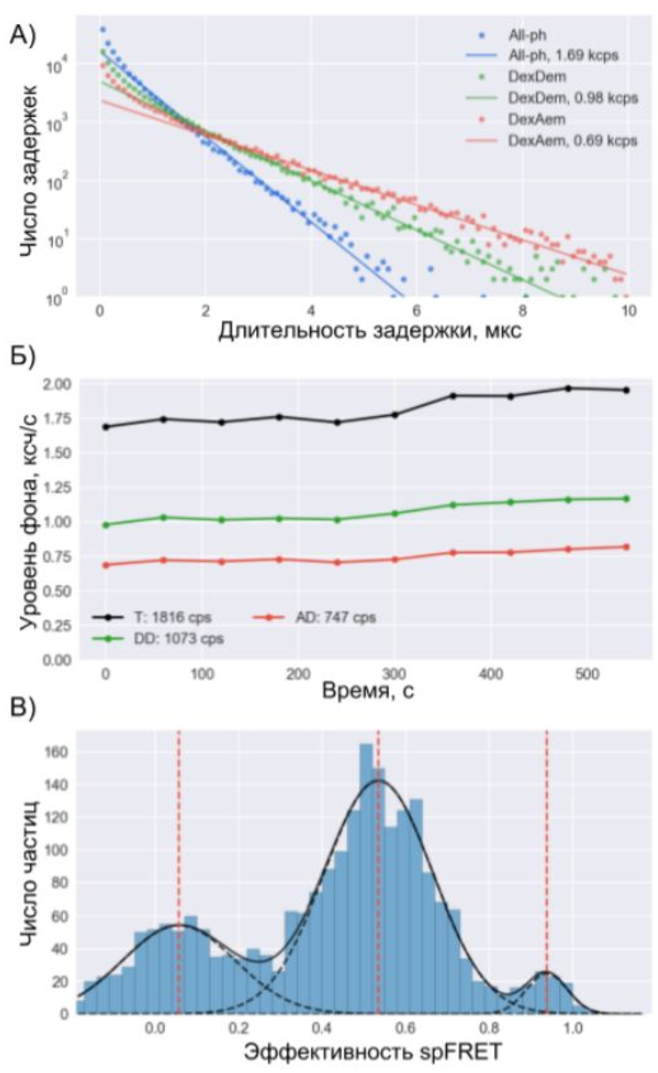
\includegraphics[width=100pt]{images/p1/part1_5_fret/part1_5_fret_f5.pdf}
%     \caption{А) гистограмма длительностей задержек между соседними фотонами в канале донора (зеленый), акцептора (красный), в обоих каналах (синий). Б) изменение уровня фона в ходе эксперимента. В) Типовая гистограмма эффективности spFRET со вписанными в нее тремя функциями Гаусса}
%     \label{fig:p1_5_fret:f5}
% \end{figure}

\subsubsection{Измерение фактора детекции}
При ратиометрическом измерении FRET вычисление истинного $E_{FRET}$ требует определения корректирующего фактора $\gamma$. Данный фактор позволяет перемасштабировать отношение регистрируемых интенсивностей сигнала в каналах донора и акцептора, чтобы учесть разницу в квантовых выходах красок и эффективности детекции фотонов от разных красок прибором. Также фактор детекции может изменяться целенаправленно варьируя параметры прибора для достижения большего разрешения в областях расстояния между метками большими или меньшими радиуса Ферстера \cite{gansen_structural_2009}. 

Для измерения параметра $\gamma$ можно использовать ряд экспериментальных методик. Квантовые выходы измеряют их сравнения с квантовыми выходами известных красителей \cite{williams_relative_1983}. Инструментальную часть фактора, $\gamma_{instrument}$, можно вычислить используя формулу:
\begin{equation}
    \gamma_{instrument} = \frac{m_{A}^{smF} m_{D}^{Abs} \Phi_{D}}{m_{D}^{smF} m_{A}^{Abs} \Phi_{A}}
\end{equation}
    где $m_{A}^{smF}$ и $m_{D}^{smF}$ - производные интенсивности флуоресценции акцептора и донора по концентрации для заданного лазера, $m_{A}^{Abs}$ и $m_{D}^{Abs}$ - производные поглощения акцептора и донора от концентрации, измеренные на длинне волны возбуждения донора, $\Phi_A$ и $\Phi_D$ квантовые выходы акцептора и донора. Более подробно методика описана в работе \cite{ferreon_interplay_2009}.

Альтернативой измерению фактора детекции в отдельных экспериментах (в том числе с применением спектрофотометра), является его измерение непосредственно во время эксперимента. Например, метод ALEX FRET (alternating laser excitation FRET) использует чередующиеся вспышки двух лазеров, возбуждающих поочередно донор или акцептор. Такой метод позволяет сразу определить стехиометрию красок в проплывающем комплексе. Измеряя эффективность переноса для комплексов с различной стехиометрией можно рассчитать фактор детекции \cite{lee_accurate_2005}. 

% \subsection{Детекция структурной гетерогенности в образце}
%     Чаще всего, результаты измерения эффективности spFRET анализируют путем построения частотных гистограмм (Рис. 5 В). Полученные распределения затем аппроксимируют Гауссовыми функциями, положение которых принимают за среднюю эффективность переноса энергии для субпопуляции частиц. Средняя эффективность переноса энергии затем может быть использована для оценки среднего расстояния между флуоресцентными метками. Помимо средней эффективности, информацию об исследуемой системе можно получить из формы и ширины распределения эффективностей spFRET [60,61]. Уширение распределений может свидетельствовать как о статической структурной гетерогенности образца, так и о динамической структурной гетерогенности образца: под статической гетерогенностью понимают наличие в образце смеси частиц с разными расстояниями между метками, изменение расстояний при этом либо не происходит, либо происходит на временах, значительно превышающих времена диффузии частиц сквозь фокальный объем. О динамической гетерогенности говорят в случае наличия конформационной подвижности молекул, приводящей к тому, что эффективность spFRET изменяется в ходе диффузии частицы сквозь фокальный объем. Возможность наблюдения динамической гетерогенности позволяет судить о характерных временах конформационных перестроек в макромолекулах.%not edited
%     В работе [62] был предложен оригинальный подход для определения наличия динамической гетерогенности в образце, основанный на определении вариабельности сигнала в процессе проплывания частицы через фокальный объем. Наличие быстрых структурных перестроек внутри образца должно приводить к увеличению стандартного отклонения измеренной эффективности spFRET для каждой детектируемой вспышки флуоресценции. В случае отсутствия подвижности в образце, отклонения в сигнале будут вызваны лишь случайным шумом, который достаточно просто оценить. Любая последовательность из $n$ фотонов в канале флуоресценции донора подчиняется биномиальному распределению с вероятностью успеха равной эффективности FRET ( $E^*=\frac{N_a}{N_a+N_d}$ , где $N_x$ - число фотонов в канале донора или акцептора, $n$ - общее число фотонов). Исходя из этого, стандартное отклонение сигнала в канале акцептора будет описываться формулой $\sigma_{Na}=\sqrt{n E^* (1-E^*)}$ , а стандартное отклонение эффективности spFRET будет подчиняться формуле%not edited
% \begin{equation}
%     \sigma_{E^*}=\sqrt{\frac{ E^* (1-E^*)}{n}}
% \end{equation}
%     Эта кривая (пунктирная линия на Рис. 6) является ориентиром для оценки стандартного отклонения исследуемого сигнала. Для каждой вспышки флуоресценции рассчитывается стандартное отклонение эффективности spFRET:%not edited
% \begin{equation}
%     \sigma_i = \sqrt{\frac{1}{N_i}\sum_{j=1}^{Ni} (\epsilon_{ij} - \mu_i)^2} , где \mu_i = \frac{1}{Ni}\sum_{j=1}^{Ni} \epsilon_{ij}
%     \end{equation}
%     и строится двумерная гистограмма распределения стандартного отклонения от величины эффективности переноса энергии (Рис. 6). При этом, если среднее стандартное отклонение превышает ожидаемое из биномиального распределения, можно говорить о наличии динамической гетерогенности в образце, которая приводит к уширению профилей эффективности spFRET.%not edited
    
%  \begin{figure} [h!]
%      \centering
%      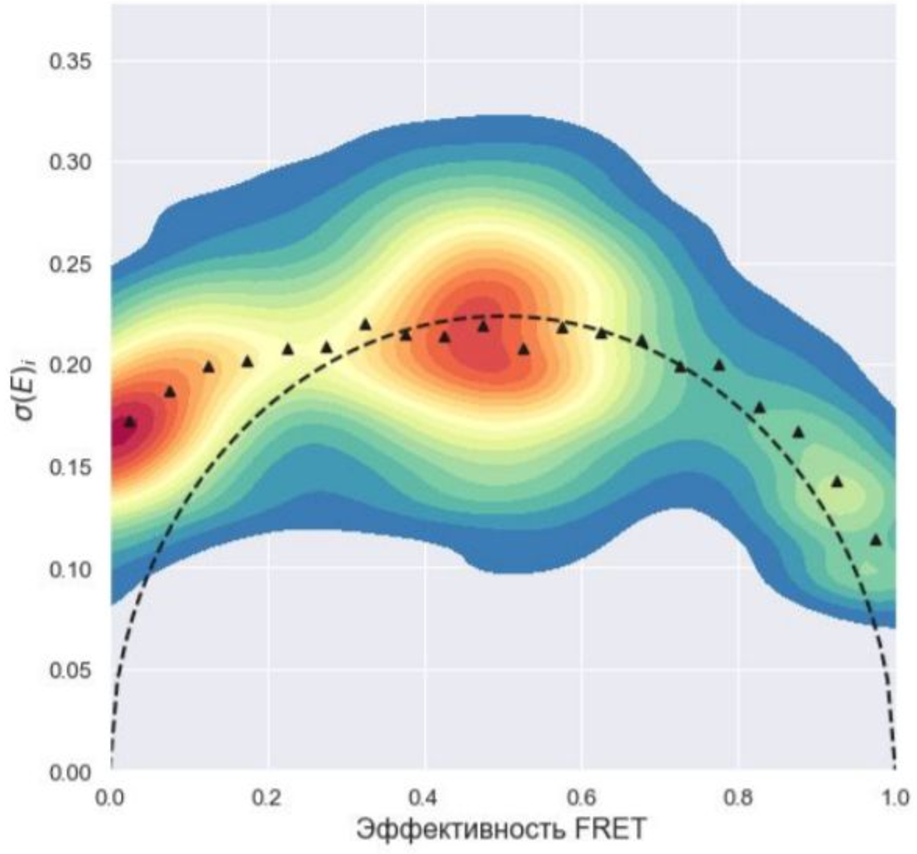
\includegraphics[width=\textwidth]{images/p1/part1_5_fret/part1_5_fret_f6.pdf}
%      \caption{Двумерная гистограмма распределения стандартного отклонения величины эффективности spFRET. Пунктиром показана линия ожидаемого стандартного отклонения для сигнала, распределенного биномиально (Формула 10).}
%      \label{fig:p1_5_fret:f6}
%  \end{figure}
 
    % На приведенной двумерной гистограмме (Рис. 6) видно, что для низких и высоких величин эффективности FRET стандартные отклонения превышают теоретическую оценку. Этот эффект может свидетельствовать о наличии быстрых перестроек в этих субпопуляциях частиц, но также может быть связан с тем, что метод оценки вариабельности вспышек не учитывает уровень фона и другие корректировочные коэффициенты (см. Формулу 3).%not edited










